% Batch size for curvature steps: three quantities. Build: see README.md in this folder.
\documentclass[11pt,a4paper]{article}

\usepackage[T1]{fontenc}
\usepackage{lmodern}
\usepackage[a4paper,margin=2.5cm]{geometry}
\usepackage{amsmath,amssymb,amsthm,mathtools}
\usepackage{graphicx}
\usepackage[shortlabels]{enumitem}
\usepackage{xcolor}
\usepackage{microtype}
\usepackage[colorlinks=true,linkcolor=blue!50!black,urlcolor=blue!50!black,citecolor=blue!50!black]{hyperref}

% Generated by make_figure.py; do not edit by hand.
\newcommand{\NumWishDraws}{20{,}000}
\newcommand{\NumWishMOne}{1.5382}
\newcommand{\NumWishMOnePred}{1.5385}
\newcommand{\NumWishMTwo}{3.6770}
\newcommand{\NumWishMTwoPred}{3.6798}
\newcommand{\NumProdSim}{0.2853}
\newcommand{\NumProdPred}{0.2856}
\newcommand{\NumShareSimHalf}{0.336}
\newcommand{\NumSharePredHalf}{0.333}
\newcommand{\NumShareSimTwo}{-0.332}
\newcommand{\NumSharePredTwo}{-0.333}
\newcommand{\NumFigD}{256}
\newcommand{\NumFigK}{2{,}000}
\newcommand{\NumFigBov}{85}
\newcommand{\NumFigBGrad}{413}
\newcommand{\NumFigBGradNumeric}{413}
\newcommand{\NumFigBBoth}{1132}
\newcommand{\NumFigKappaAtBGrad}{0.38}
\newcommand{\NumFigSurvAtBGrad}{0.17}
\newcommand{\NumLabSlope}{2.2}
\newcommand{\NumLabIntercept}{14}
\newcommand{\NumLabBov}{66}


\DeclareMathOperator{\tr}{tr}
\DeclarePairedDelimiter{\norm}{\lVert}{\rVert}
\newcommand{\E}{\mathbb{E}}
\newcommand{\Bov}{B_{\mathrm{ov}}}
\newcommand{\study}[1]{\path{#1}}

\theoremstyle{plain}
\newtheorem{proposition}{Proposition}
\newtheorem{lemma}[proposition]{Lemma}
\theoremstyle{definition}
\newtheorem{approximation}[proposition]{Approximation}
\theoremstyle{remark}
\newtheorem{remark}[proposition]{Remark}

\title{Batch size for curvature steps: three quantities\\[0.3em]
\large Derivations, background, and why they might matter}
\author{Working note --- G.~Tirpitz and Claude (Opus 5.5)}
\date{23 October 2026}

\begin{document}
\maketitle

\noindent\textbf{Question.} At which batch size does an exact (layerwise) GGN step stop overfitting its batch, while
keeping the advantage the quadratic model promises? This note derives three quantities that answer it: a
noise-to-signal ratio $r$ that decides both overfitting and how much of the advantage survives
(Section~\ref{sec:r}); a compute-optimal batch size once steps have a price (Section~\ref{sec:cost}); and the noise
in the curvature estimate itself, which classical batch-size theory leaves out (Section~\ref{sec:curv}).
Section~\ref{sec:together} combines them, and Section~\ref{sec:next} lists what to investigate. Statements are
exact unless labelled as approximations; all numbers marked as checks come from \texttt{make\_figure.py} in this
folder.

\section{Setting}

Near the current weights $w$, model the corpus loss by a quadratic,
\[
L(w)=L^*+\tfrac12(w-w^*)^\top H(w-w^*),\qquad g=H(w-w^*),\qquad \Delta L=L(w)-L^*=\tfrac12\,g^\top H^{-1}g .
\]
A batch of $B$ examples drawn without replacement from $N$ gives $g_B=g+\xi$ with $\E\xi=0$ and
$\operatorname{Cov}\xi=(\tfrac1B-\tfrac1N)\Sigma$, where $\Sigma$ is the covariance of per-example gradients. A
preconditioned step is $w^+=w-\alpha Pg_B$ with $P$ symmetric positive definite. The exact Newton (GGN) step is
$P=H^{-1}$; for least squares the GGN equals $H$. For Newton it helps to whiten: with $u=H^{1/2}(w-w^*)$ the loss is
$\Delta L=\frac12\norm{u}^2$, the whitened gradient is $u$, and the whitened noise is $\zeta=H^{-1/2}\xi$.

%======================================================================
\section{Quantity 1: the ratio $r$, overfitting, and what survives}\label{sec:r}
%======================================================================

\begin{proposition}[Step size tuned in expectation]\label{prop:tuned}
For fixed $P$, the best expected decrease of the corpus loss is
\[
\max_\alpha \E\bigl[L(w)-L(w^+)\bigr]=\frac{\Phi_P}{1+r_P},\qquad
\Phi_P=\frac{(g^\top Pg)^2}{2\,g^\top PHPg},
\]
\[
r_P=\Bigl(\frac1B-\frac1N\Bigr)K_P,\qquad
K_P=\frac{\tr(PHP\Sigma)}{g^\top PHPg}.
\]
\end{proposition}
\begin{proof}
$L(w)-L(w^+)=\alpha g^\top Pg_B-\frac12\alpha^2 g_B^\top PHPg_B$. Taking expectations with $\E g_B=g$ and
$\E[g_B^\top Mg_B]=g^\top Mg+\tr(M\operatorname{Cov}\xi)$ gives
$\alpha\,g^\top Pg-\frac12\alpha^2\bigl(g^\top PHPg+\tr(PHP\operatorname{Cov}\xi)\bigr)$; maximize over $\alpha$.
\end{proof}

$\Phi_P$ is what the quadratic model promises for the direction without noise; $K_P$ is the step's
\emph{noise scale}, in examples. For Newton, $\Phi=\Delta L$ (the noiseless Newton step solves the quadratic), and
\[
\text{share kept}=\frac{1}{1+r},\qquad r=\Bigl(\frac1B-\frac1N\Bigr)K_1,\qquad K_1=\frac{\tr(H^{-1}\Sigma)}{2\,\Delta L}.
\]
For least squares with label noise $\sigma^2$, near the optimum $\Sigma\approx\sigma^2H$ and therefore
$K_1\approx D\sigma^2/(2\Delta L)$: the noise scale grows as the loss falls.

\begin{approximation}[Step size fitted on the step's own batch]\label{approx:share}
Let $\hat\alpha$ minimize the batch's own quadratic model along $Pg_B$ (with the exact curvature $H$). The share of
the decrease the batch model predicts that the corpus actually sees is exactly
$s=2\,g^\top Pg_B/(g_B^\top Pg_B)-1$. Replacing numerator and denominator by their expectations,
\[
s\approx\frac{1-\tilde r}{1+\tilde r},\qquad \tilde r=\frac{\tr(P\operatorname{Cov}\xi)}{g^\top Pg},
\]
and $\tilde r=r$ for Newton. Check (whitened Newton, $D=200$): $r=\tfrac12$ gives $\NumShareSimHalf$ against
$\NumSharePredHalf$; $r=2$ gives $\NumShareSimTwo$ against $\NumSharePredTwo$.
\end{approximation}
\begin{proof}[Derivation of the exact form]
The fitted step size is $\hat\alpha=g_B^\top Pg_B/(g_B^\top PHPg_B)$, and the batch-predicted decrease is
$\frac12\hat\alpha\,g_B^\top Pg_B$. The corpus decrease is
\[
\hat\alpha\,g^\top Pg_B-\tfrac12\hat\alpha^2g_B^\top PHPg_B=\hat\alpha\,g^\top Pg_B-\tfrac12\hat\alpha\,g_B^\top Pg_B .
\]
Divide the second by the first.
\end{proof}

\paragraph{Reading.} One ratio decides both questions in the opening sentence.
\begin{itemize}[nosep]
\item \emph{Overfitting:} for $r>1$, i.e.\ $B\lesssim K_1$, a Newton step whose length is fitted on its own batch
  \emph{increases} the corpus loss in expectation.
\item \emph{Advantage kept:} with a step size chosen in expectation (or on a second batch), a fraction $1/(1+r)$ of
  the promised gain survives.
\end{itemize}

\paragraph{Background.} For $P=I$ this is McCandlish et al.'s noise scale: the best progress per step is
$\Delta L_{\max}/(1+B_{\mathrm{noise}}/B)$, and the trade-off between steps and examples has its knee near
$B_{\mathrm{noise}}$. Zhang et al.'s noisy quadratic model showed that preconditioning raises the batch size up to
which larger batches help. The share law of Approximation~\ref{approx:share} is the lab's transfer law (N16/N20 in
\path{ideas/batch_noise.md}): on MNIST it predicted measured shares with Spearman 0.963. It overstated the harm for
the exact GGN at small $B$, where the batch's curvature along the fitted step exceeds the corpus curvature, so the
search limits itself.

\paragraph{Why it matters here.} In \study{noise_scale_20261021} (CIFAR, whitened per-tensor GGN), $r$ at
$B=2{,}048$ was 0.63--1.01 at step 10 and 8.1--9.5 at step 400. So in theory about half of the Newton advantage
survives early and about a tenth late; the measured gains were smaller still. This is the lab's rule ``curvature pays
early, not late'' as a formula. Because $K_P$ grows with the strength of $P$, it also explains why the best power of
the curvature is fractional.

%======================================================================
\section{Quantity 2: the compute-optimal batch}\label{sec:cost}
%======================================================================

The share $1/(1+r)$ improves with $B$ indefinitely, so ``the right batch size'' needs a price. Let one step cost
$c(B)=c_{\mathrm{step}}+c_{\mathrm{ex}}B$: a fixed part per step (building and factorizing curvature, solves,
overheads) and a part per example. Write $\Bov=c_{\mathrm{step}}/c_{\mathrm{ex}}$, the per-step overhead in units of
examples.

\begin{proposition}[Compute-optimal batch]\label{prop:cost}
For $N\to\infty$ and fixed $P$, the expected progress per unit compute,
$\pi(B)=\Phi_P/\bigl((1+K_P/B)(c_{\mathrm{step}}+c_{\mathrm{ex}}B)\bigr)$, is maximized at
\[
B^*=\sqrt{K_P\,\Bov},\qquad\text{where the share kept is }\frac{1}{1+\sqrt{K_P/\Bov}} .
\]
\end{proposition}
\begin{proof}
$\pi\propto 1/h(B)$ with $h(B)=(1+K/B)(c_{\mathrm{step}}+c_{\mathrm{ex}}B)
=c_{\mathrm{step}}+c_{\mathrm{ex}}K+c_{\mathrm{ex}}B+Kc_{\mathrm{step}}/B$. Then
$h'(B)=c_{\mathrm{ex}}-Kc_{\mathrm{step}}/B^2=0$ at $B^2=Kc_{\mathrm{step}}/c_{\mathrm{ex}}$, and $h$ is convex
for $B>0$.
\end{proof}

\begin{remark}\leavevmode
\begin{enumerate}[(a),nosep]
\item A step with almost no per-step overhead ($\Bov\approx0$, plain SGD) wants small batches; a step that pays a
  lot per step wants larger ones. The optimum is the geometric mean of the noise scale and the overhead.
\item For a dense Newton step on a $D$-dimensional block, $c_{\mathrm{ex}}\approx D^2$ (accumulating the curvature)
  and $c_{\mathrm{step}}\approx D^3/3$ (Cholesky), so $\Bov\approx D/3$. For least squares this gives
  $B^*\approx D\sigma/\sqrt{6\Delta L}$: the compute-optimal batch grows as the excess loss falls, i.e.\ the theory
  asks for a growing batch schedule.
\item Lab costs are measurable: a full-GGN product in \study{bulk_krylov_20261014} took 0.070\,s at 256 examples and
  0.46\,s at 2{,}048. A line through these two points gives about \NumLabIntercept\,ms fixed plus
  $\NumLabSlope\times10^{-4}$\,s per example, so the fixed part equals about \NumLabBov{} examples (two data points;
  an illustration only).
\end{enumerate}
\end{remark}

\paragraph{Background and why it matters.} This is a two-line consequence of McCandlish et al.'s trade-off with an
explicit price per step; it is elementary and probably stated somewhere. Its use here is that it turns ``what does
curvature cost'' (the Hennig route) into a batch-size rule, and the growth of $K_1$ during training (the Orvieto
route, where the noise scale acts as a temperature) into a batch schedule. It is also the natural target of the
derivative-free homework: a compute-limited run whose optimum the theory predicts.

%======================================================================
\section{Quantity 3: noise in the curvature itself}\label{sec:curv}
%======================================================================

A GGN optimizer does not know $H$; it estimates it from a batch. Classical batch-size theory, including both
references above, treats the curvature as known. Take least squares with Gaussian inputs $x\sim\mathcal N(0,H)$ and
curvature $\hat H=\frac1n\sum_{i\le n}x_ix_i^\top$ from $n$ examples. In whitened coordinates
$\hat S=H^{-1/2}\hat H H^{-1/2}$, and $n\hat S$ is a Wishart matrix with $n$ degrees of freedom and identity scale.

\begin{lemma}[Inverse-Wishart moments; e.g.\ Gupta \& Nagar 2000]\label{lem:wishart}
For $n>D+3$,
\[
\E[\hat S^{-1}]=m_1I,\quad m_1=\frac{n}{n-D-1};\quad
\E[\hat S^{-2}]=m_2I,\quad m_2=\frac{n^2(n-1)}{(n-D)(n-D-1)(n-D-3)} .
\]
\vspace{-0.5\baselineskip}
Check ($D=20$, $n=60$, \NumWishDraws{} draws): $m_1$ \NumWishMOne{} against \NumWishMOnePred, $m_2$ \NumWishMTwo{}
against \NumWishMTwoPred.
\end{lemma}

So the batch Newton step is too long on average, by $n/(n-D-1)$, and its spread blows up as $n$ approaches $D$:
the smallest eigenvalues of a sample covariance are underestimated, and the inverse amplifies them.

\begin{proposition}[Both noise channels]\label{prop:both}
Take the Newton direction with curvature $\hat S$ from $n$ examples and a gradient from an independent batch with
ratio $r$ (Section~\ref{sec:r}). With the best step size, the expected fraction of $\Delta L$ removed is
\[
\frac{\kappa(n,D)}{1+r},\qquad \kappa(n,D)=\frac{m_1^2}{m_2}=\frac{(n-D)(n-D-3)}{(n-D-1)(n-1)} .
\]
Check ($D=50$, $n=120$, $r=1$): \NumProdSim{} simulated against \NumProdPred.
\end{proposition}
\begin{proof}
In whitened coordinates the step is $u^+=u-\alpha\hat S^{-1}(u+\zeta)$, with $\zeta$ independent of $\hat S$,
$\E\zeta=0$ and $\E\norm{\zeta}^2=r\norm{u}^2$. By Lemma~\ref{lem:wishart} and independence,
$\E\norm{u^+}^2=\norm{u}^2\bigl(1-2\alpha m_1+\alpha^2m_2(1+r)\bigr)$. The minimum over $\alpha$ is
$\norm{u}^2\bigl(1-m_1^2/(m_2(1+r))\bigr)$.
\end{proof}

\begin{remark}\leavevmode
\begin{enumerate}[(a),nosep]
\item $\kappa\approx(n-D-2)/(n-1)\approx1-D/n$ for $n\gg D$: curvature noise acts like a second noise scale of
  about $D$ examples, and the two channels multiply. As $n$ falls to $D+3$, $\kappa\to0$: below about $D$ examples
  per block, an undamped Newton step gains nothing even with the best step size.
\item \emph{GGN heuristic.} One example contributes rank at most $C-1$ to a GGN with $C$ outputs, so the threshold
  is roughly $n\approx D/(C-1)$. For the lab's $64\times256$ MLP blocks ($D=16{,}384$, $C=10$) that is about
  1{,}820 examples, close to the training batch of 2{,}048. This is a heuristic: GGN rows are not Gaussian, confident
  predictions shrink the effective rank, and damping changes the picture near the threshold.
\item \emph{Fractional powers.} The mean of $s^{-\nu}$ over the sample spectrum increases with $\nu$, so curvature
  noise penalizes $\nu=1$ more than $\nu=\frac12$. That is the direction of the noise-scale study's miss: its theory
  treated the curvature as exact and overstated the gains by 1.5--3.8$\times$ at $\nu=\frac12$ and 2--9$\times$ at
  $\nu=1$.
\end{enumerate}
\end{remark}

\paragraph{Background and why it matters.} The underestimated small eigenvalues are the Marchenko--Pastur picture of
sample covariances. In optimization, Tatzel et al.\ (2025) show that mini-batch quadratics are systematically
biased, the same phenomenon seen from the quadratic model's side. Of the three quantities this is the one least
covered by standard batch-size theory: it has its own threshold, independent of gradient noise, and it is specific to
curvature methods. It is a candidate explanation for the open question of why the noise-scale theory was too
optimistic (open test 6 in \path{ideas/batch_noise.md}).

%======================================================================
\section{Putting them together}\label{sec:together}
%======================================================================

\begin{figure}[h]
\centering
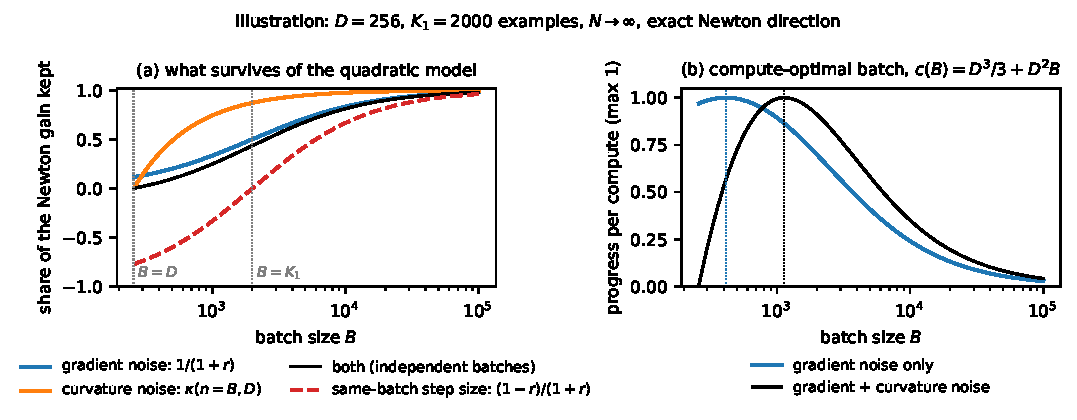
\includegraphics[width=\linewidth]{figures/survival_cost.pdf}
\caption{Illustration with $D=\NumFigD$, $K_1=\NumFigK$, $N\to\infty$, exact Newton direction. (a) Share of the
Newton gain kept: gradient noise (Proposition~\ref{prop:tuned}), curvature noise with $n=B$
(Proposition~\ref{prop:both}), both from independent batches, and the share with a step size fitted on the batch
(Approximation~\ref{approx:share}). (b) Progress per unit compute with $c(B)=D^3/3+D^2B$, i.e.\ $\Bov\approx\NumFigBov$.}
\label{fig:together}
\end{figure}

In the illustration of Figure~\ref{fig:together}, gradient noise alone puts the compute-optimal batch at
$B^*=\sqrt{K_1\Bov}=\NumFigBGrad$ (numerical maximum \NumFigBGradNumeric). There only \NumFigSurvAtBGrad{} of the
gain survives the gradient noise, and curvature noise from a batch of that size keeps only \NumFigKappaAtBGrad{}
of the rest. With both channels the optimum moves to about \NumFigBBoth, a few multiples of $D$. Curvature noise
thus pushes the compute-optimal batch of a curvature method up, toward the block dimension. The figure assumes
independent batches for gradient and curvature; the case of one batch for both is not covered by these formulas.

%======================================================================
\section{What to investigate}\label{sec:next}
%======================================================================

\begin{enumerate}[nosep]
\item \textbf{Synthetic least squares.} Verify Proposition~\ref{prop:both} with independent batches, then use one
  batch for gradient and curvature ($n=B$, correlated; the step becomes the batch's own least-squares solution), then
  add damping $\delta$. How should the best $\delta$ scale with $D/n$?
\item \textbf{Compute-optimal batch by derivative-free search} (the homework). Inputs $\log B$, $\log\delta$,
  $\log\eta$ under a fixed compute budget; compare the optimum found with Proposition~\ref{prop:cost} and
  Figure~\ref{fig:together}.
\item \textbf{Curvature channel in the lab} (open test 6). Replay noise-scale states with the curvature estimated
  from $n\in\{1{,}000,\,4{,}000,\,16{,}000\}$ reference examples. Does the theory's optimism shrink as $n$ grows?
\item \textbf{Cost in the lab.} Measure $c_{\mathrm{step}}$ and $c_{\mathrm{ex}}$ for an actual curvature step,
  predict $B^*(t)$ from the measured $K_1(t)$, and test a growing batch schedule against a constant $B=2{,}048$ at
  equal compute.
\item \textbf{Averaging.} The lab's optimizers average statistics over steps. An average over $k$ steps lowers the
  noise roughly $k$-fold but adds staleness; fold this into all three quantities (T4 in
  \path{ideas/batch_noise.md}).
\end{enumerate}

\begin{thebibliography}{9}\setlength{\itemsep}{2pt}\small
\bibitem{gupta} A.~K.~Gupta and D.~K.~Nagar. \emph{Matrix Variate Distributions}. Chapman \& Hall/CRC, 2000. (Cited
  from memory; the two moments in Lemma~\ref{lem:wishart} were checked numerically.)
\bibitem{mccandlish} S.~McCandlish, J.~Kaplan, D.~Amodei et al. An empirical model of large-batch training.
  arXiv:1812.06162, 2018. (Cited from memory.)
\bibitem{tatzel} L.~Tatzel, B.~Mucs\'anyi, O.~Hackel and P.~Hennig. Debiasing mini-batch quadratics for applications in
  deep learning. \emph{ICLR}, 2025. arXiv:2410.14325. (Checked online 23 October 2026.)
\bibitem{zhang} G.~Zhang, L.~Li, Z.~Nado, J.~Martens, S.~Sachdeva, G.~Dahl, C.~Shallue and R.~Grosse. Which
  algorithmic choices matter at which batch sizes? Insights from a noisy quadratic model. \emph{NeurIPS}, 2019.
  arXiv:1907.04164. (Cited from memory.)
\bibitem{lab} Lab notes: \path{ideas/batch_noise.md} (T1, T7, R3, open test 6);
  \path{studies/noise_scale_20261021/RESULTS.md}; \path{studies/bulk_krylov_20261014/RESULTS.md} (K5).
\end{thebibliography}

\end{document}
